\documentclass[12pt]{article}
\usepackage[utf8x]{inputenc}
\usepackage{amsmath}
\usepackage{graphicx}
\usepackage{indentfirst}
\usepackage[super]{natbib}
\usepackage{float}
\usepackage{amssymb}
\usepackage[version=4]{mhchem}
%\usepackage{hyperref}



\title{Pattern Formation in Lung Development}
\author{Geneva Porter}
\date{16 May, 2019}

\begin{document}

\begin{titlepage}
\maketitle
\thispagestyle{empty}

\begin{center}
	
\large \it San Diego State University 
	
Professor C Curtis

\end{center}
\end{titlepage}

\tableofcontents

\section{Introduction and Motivation}\label{introduction}

\subsection{Biological Background}\label{bio}

In 1952, Alan Turing published his highly influential work {\it The Chemical Basis of Morphogenesis},\cite{Turing1952} which changed our understanding of theoretical biology. Turing discussed how biological patterns can arise from chemical disturbances in biological homogeneous systems. He states that phenomena such as skin pigmentation patterns can be explained by chemical reaction-diffusion systems occurring as early as the embryonic stage of development. 

Without disturbances in a spatially homogeneous reaction-diffusion system, there can be no deviation from the uniform sphere. While this describes many organisms very early in development, deviations from homogeneity are needed to spark morphogenesis and form organs, limbs, and eventually, skin patterns. Turing noted that these disturbances can be described as unstable equilibria; a small deviation from the homogeneous state will interrupt the system from developing uniformly. He also noted that such equilibria are not observed to exist {\it per se} in nature, but rather occur when the disturbance in a systems causes a stable equilibrium to become unstable. This phenomenon is known as a {\it Turing Instability}, and is observed in mathematical systems with the addition of a diffusion term.

Several notable works have since adapted and expanded Turing's model.\cite{Gierer1972}\cite{Lee2000}\cite{Krause2018} This paper will investigate one such model, proposed by Schnakenberg in his 1979 work {\it Simple Chemical Reaction Systems With Limit Cycle Behavior}.\cite{Schnakenberg1979} The Schnakenberg model, also known as the activator-depletion model, is characterized by the kinetics of two reacting morphogens exhibiting auto-catalytic behavior. 

We will apply Turing's theory and Schnakenberg's model to branch patterning in the developing lung. Current biological research has not revealed the deciding factors in branching morphogenesis that determine branch type, location, and orientation.\cite{Menshykau2012} However, we do know that two gene proteins, Fibroblast Growth Factor 10 (FGF10) and Sonic Hedgehog (SHH), are crucial to lung development.\cite{Schittny2017} FGF10 stimulates tissue growth, while SHH inhibits it. One theory proposes that branching patterns occur from the genetic expression of FGF10 and SHH {\it outside} the lung, in a fluid-filled region called the mesenchyme.\cite{Roth-Kleiner2003} These expressions can theoretically form concentration patterns on the lung surface and diffuse inward, thus determining branching morphogenesis.

An analysis of the Schnakenberg model in this context may give insight into genes interact during development, and could lead to several medical applications. I will examine this model on the surface of a sphere, and offer an analytic solution. This analysis will first provide a few key definitions and models that will be referenced throughout the paper, then perform a stability analysis when there is no diffusion. We can then include the diffusion terms along with a small perturbation from the fixed points, and determine which parameters give rise to instabilities in this context. In theory, substituting these parameters into the model and then solving on some n-dimensional geometry will result in regions of concentrated substrates. The goal of this paper is to establish a foundation for future work on lung branching morphogenesis. 

\subsection{Turing's Classic Reaction-Diffusion Model}\label{classic_model}

The original basis for Turing's model is the interaction of two substances that undergo chemical reactions and spatial diffusion. This classic reaction-diffusion system has the general form:

\begin{equation}
\label{eq:classic}
    \begin{aligned}
    &\dot{u}=D_u\Delta u+\overbrace{f(u,v)}^\text{reaction} \\
    &\dot{v}=\underbrace{D_v\Delta v}_\text{diffusion}+g(u,v)
    \end{aligned}
\end{equation}
\\
\noindent Both $u$ and $v$ are functions of position and time. Also, $f(u,v)$ and $g(u,v)$ describe the concentration of the reactants, as well as the rates of production and degradation of the products. The $\Delta$ terms represent the diffusion behavior in the system, with diffusion rates $D_u$ and $D_v$. 


\subsection{Schnakenberg's Activator-Depleated Substrate Model}\label{schnakenberg}

Let us consider Schnakenberg's approach. He considered the kinetics of a tri-molecular reaction, given by:

$$ X\ce{ <=>[k_1][k_2] F} ~~~~~~~~ \text{2F}+\ce{S ->[k_3] 3F} ~~~~~~~~ Y\ce{->[k_4] S} $$

\noindent Here, F represents the activator FGF10, and S represents the inhibitor SHH. X and Y are their respective precursor substrates. Using the law of mass action, this series of reactions is represented by Equation (\ref{eq:Schnakenburg}) below. Let the function $F(\rho,\phi,\theta,t)$ designate the behavior of FGF10, while $S(\rho,\phi,\theta,t)$ applies to SHH. This model is then given by:
\\
\begin{equation}
\label{eq:Schnakenburg}
    \begin{aligned}
    \dot{F} & = D_F\Delta F + k_1 - k_2F + k_3F^2S \\
    \\
    \dot{S} & = D_S\Delta S + k_4 - k_3F^2S \\
    \end{aligned}
\end{equation}
\\
\noindent All parameters are positive and real. Initial amounts of FGF10 and SHH are given by $k_1$ and $k_4$, respectively. The activator FGF10 is created auto-catalytically, represented by the terms $k_3F^2S$ (positive auto-catalysis with SHH) and $k_2F$ (negative auto-catalysis with the precursor substrate). The $k_3F^2S$ term subtracted from the inhibitor equation for SHH, since the SHH decreases in concentration as FGF10 is produced during the $k_3$ reaction. The two morphogens form a feedback loop that ensures a cyclic production and degradation of each substance when in the steady-state. Like the classic Turing model, the diffusion of the substances in the domain is given by the Laplacian terms in each equation, with diffusion rates $D_F$ and $D_S$.

\subsection{The Laplace-Beltrami Operator}\label{laplace-beltrami}

Since this project is only examining the surface of a sphere, Laplace operator in Schnakenberg's model will be replaced with the Laplace-Beltrami operator. There are a few groups that have already sucessfully investigated this method of solving a Turing model on surface geometries.\cite{Dziuk1988}\cite{Shubin2001}\cite{Barreira2011} 

Let $\Omega$ be an open subset in $\mathbb{R}^3$ and $\Gamma$ be a hypersurface contained in $\Omega$. The Laplace-Beltrami operator is given by:
\\
\begin{equation}
    \label{Laplace-Beltrami}
    \begin{aligned}
        \Delta_\Gamma u = \nabla_\Gamma\cdot\nabla_\Gamma u ~~~~~ \text{with} \\
        \\
        \nabla_\Gamma u = \nabla u-(\nabla u\cdot\vec{n})\vec{n}
    \end{aligned}
\end{equation}
\\
\noindent Here, $\nabla_\Gamma u$ is the tangential gradient, and $\vec{n}$ is the normal unit vector. We can see that the surface Laplacian is the divergence of the tangential gradient. This operation is readily done in spherical coordinates, as it simply eliminates the dependence on the radius.

\pagebreak
\section{Stability Without Diffusion}\label{stability}

\subsection{Nondimensionalization}\label{nondimensionalization}

To more easily perform this analysis, we can begin by nondimensionalizing the parameters and replacing the diffusion terms with the surface Laplacian. Referencing equation (\ref{eq:Schnakenburg}), we can use the following substitutions:
$$ F = \tilde{F}F_a ~~~~~ S = \tilde{S}S_a ~~~~~  \vec{x} = \hat{x}x_a ~~~~~  t = \tau t_a ~~~~~ \Delta\rightarrow\Delta_\Gamma$$
\noindent This results in the following equation, where the time derivative is taken with respect to $\tau$:
\begin{align*}
   &\dot{\tilde{F}} = \frac{D_Ft_a}{x_a^2}\Delta_\Gamma\tilde{F} + 
   \frac{k_1t_a}{F_a} - k_2t_a\tilde{F} + k_3F_aS_at_a\tilde{F}^2\tilde{S} \\
   &\dot{\tilde{S}} = \frac{D_St_a}{x_a^2}\Delta_\Gamma\tilde{S} +
    \frac{k_4t_a}{S_a} - k_3F_a^2t_a\tilde{F}^2\tilde{S} 
\end{align*} 
\noindent We can then make substitutions for each term, and define some new ones:
$$  F_a =  \sqrt{\frac{k_2}{k_3}} ~~~~~ S_a = \sqrt{\frac{k_2}{k_3}} ~~~~~ x_a^2 = \frac{D_F}{k_2} ~~~~~ t_a = \frac{1}{k_2} $$
$$ \text{and} ~~~ \alpha = \frac{k_1}{k_2}\sqrt{\frac{k_3}{k_2}} ~~~~~ \beta = \frac{k_4}{k_2}\sqrt{\frac{k_3}{k_2}} ~~~~~ \delta = \frac{D_S}{D_F} ~~~~~ \gamma = \frac{1}{k_2} $$
\noindent This gives us the simplified system:
\begin{equation}
\label{eq:simplified}
\begin{aligned}
    & \dot{\tilde{F}} = \Delta_\Gamma\tilde{F} + 
     f(\tilde{F},\tilde{S}) ~~~~~\text{with} ~~~~~ f(\tilde{F},\tilde{S}) = \gamma\left(\alpha - \tilde{F} + \tilde{F}^2\tilde{S}\right) \\
    & \dot{\tilde{S}} = \delta\Delta_\Gamma\tilde{S} + 
    s(\tilde{F},\tilde{S}) ~~~~~\text{with} ~~~~~ s(\tilde{F},\tilde{S}) = \gamma\left(\beta - \tilde{F}^2\tilde{S}\right) \\
\end{aligned}
\end{equation}
We now have scaled equations, and although the $\gamma$ term could have been excluded, it is useful as a scaling measure of the general strength of the reactions. For now, it is sufficient to note that the auto-catalytic terms are otherwise coefficient-less, and the rates of production and degradation of the morphogens rely on the initial concentration values of $\alpha$ and $\beta$.

\pagebreak
\subsection{Fixed Points and Stability}\label{fixed_points}
We can see from Equation (\ref{eq:simplified}) that the system relies on parameters $\alpha$ and $\beta$ to determine stability regions. We can find these regions by first removing the diffusion terms, then revealing the fixed points of the system, which are the solutions to the equations:

\begin{align*}
    & \alpha - \tilde{F} + \tilde{F}^2\tilde{S} = 0 ~~~~~~~~ \text{and} ~~~~~~~~\beta - \tilde{F}^2\tilde{S} = 0.
\end{align*}

\noindent This system has a fixed point at $(F^*,S^*)=(\alpha+\beta,\frac{\beta}{(\alpha+\beta)^2})$. To determine the region of stability about these fixed points, we first perturb the system by some small $|\varepsilon|<<1$.

\begin{equation*}
    \begin{aligned}
    F = F^*+\varepsilon~\tilde{F} ~~~~~\longrightarrow~~~~~& \dot{\tilde{F}} = \varepsilon~\tilde{F}_t = \gamma~f(F^*+\varepsilon~\tilde{F})\\
    S = S^*+\varepsilon~\tilde{S} ~~~~~\longrightarrow~~~~~& \dot{\tilde{S}} = \varepsilon~\tilde{S}_t = \gamma~s(S^*+\varepsilon~\tilde{S})
    \end{aligned}
\end{equation*}
\\
\noindent Next, a Taylor expansion about the fixed point yields:
\\
 \begin{equation}
    \left(\begin{aligned}
    \tilde{F}_t \\
    \tilde{S}_t
\end{aligned}\right)
=
\gamma\left(\begin{aligned}
    f_F(F^*,S^*) ~~~~~& f_S(F^*,S^*)\\
    s_F(F^*,S^*) ~~~~~& s_S(F^*,S^*) \\
\end{aligned}\right)
\cdot
\left(\begin{aligned}
    \tilde{F} \\
    \tilde{S}
\end{aligned}\right)
+ \mathcal{O}(\varepsilon^2)
\end{equation}
\\
\noindent Or more simply, without higher order terms:
\begin{equation}
    \label{eq:W_short}
    \dot{W}=\gamma J W
\end{equation}

\noindent Before plugging in the partial derivatives and parameters into $J$, there are some useful generalizations to highlight. Solving the linear equation $\det(J-\lambda I)$ will reveal the necessary constraints for stability:

$$
    \det \left( \begin{matrix}
    f_F-\lambda & f_S \\
    s_F & s_S-\lambda
\end{matrix} \right) = 0 ~~~~~\longrightarrow ~~~~~ \lambda^2 - \lambda\text{tr}(J) + \det(J) = 0
$$ 

\noindent It is assumed that the partial derivatives of $f$ and $s$ are evaluated at the fixed point. The the solution is:

\begin{equation}
\label{eq:lambda}
\lambda = \frac{\text{tr}(J) \pm \sqrt{\text{tr}(J)^2-4\det(J)}}{2} 
\end{equation}

\noindent Since stability is desired, we have constraints on the values for tr$(J)$ and $\det(J)$. This requires $\text{re}(\lambda)<0$, which implies $\text{tr}(J)<0$ and $\det(J)>0$. These constraints are satisfied when:
\\
\begin{equation}
    \label{eq:constraints_generic}
    f_F+s_S < 0 ~~~~~~~~~~ \text{and} ~~~~~~~~~~ f_fs_s-f_ss_F>0 
\end{equation}
\\
\noindent Now it is useful to fill in the partial derivative and parameter values. The Jacobian is therefore:

\begin{equation}
\label{eq:J}
    J =  \left.\left(
\begin{aligned}
    &-1+2FS & F^2~ \\
    &~~-2FS &~ -F^2
\end{aligned} \right)\right|_{(F^*,~S^*)} = \left(
\begin{aligned}
    -1+\frac{2\beta}{\alpha+\beta} ~~&~~~~ (\alpha+\beta)^2 \\
    -\frac{2\beta}{\alpha+\beta} ~~~~&~~ -(\alpha+\beta)^2
\end{aligned} \right)
\end{equation} 
\\
\noindent This defines the constraints as:
\\
\begin{equation}
\label{eq:constraints_w/oDiffusion}
    \beta-\alpha < (\alpha+\beta)^3 ~~~~~~~~~~ \text{and} ~~~~~~~~~~ (\alpha+\beta)^2>0
\end{equation}
\\
\noindent The second constraint is already fulfilled for all real values of $\alpha$ and $\beta$. Now we have a starting point for the Turing Instability region.  

\subsection{Bifurcation and Stable Regions}\label{bifurcation}

The constraints given in (\ref{eq:constraints_w/oDiffusion}) provide the necessary criteria for a stable region. We can visualize this stable region by noting that its border is defined by a Hopf bifurcation at tr($J$)=0. Figure (\ref{fig:stability_region}) below shows a visualization of stable and unstable regions in terms of $\alpha$ and $\beta$. We can see that a rough generalization for a stability region is given by:
\\
$$ \alpha > \frac{1}{3\sqrt{3}} ~~~~~~~ \text{and} ~~~~~~~ \beta \geq 1 $$
\\
The phase plane in Figures (\ref{fig:phase_plane}) and (\ref{fig:phase_plane2}) verify that the fixed point is stable for the parameter values $(\beta,\alpha)=(0.2,1.2)$ in the desired region, and unstable for the pair (0.05, 0.7) outside that region. We will discuss the parameter dynamics more fully in Section \ref{eigenvalue}.

\begin{figure}[H]
    \centering
    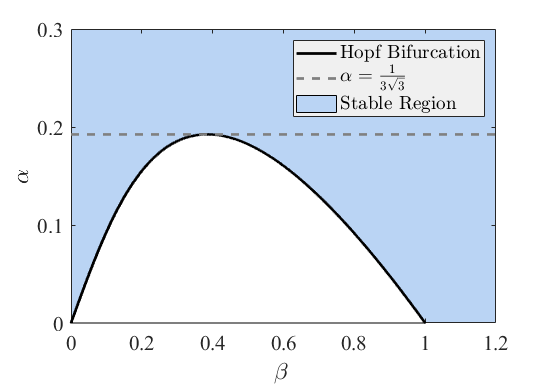
\includegraphics[width = 10cm,trim=5pts 1pts 5pts 17pts, clip]{images/stability_region.png}
    \caption{Stability region for parameters $\alpha$ and $\beta$.}
    \label{fig:stability_region}
\end{figure}

\vfill

\begin{figure}[H]
    \centering
    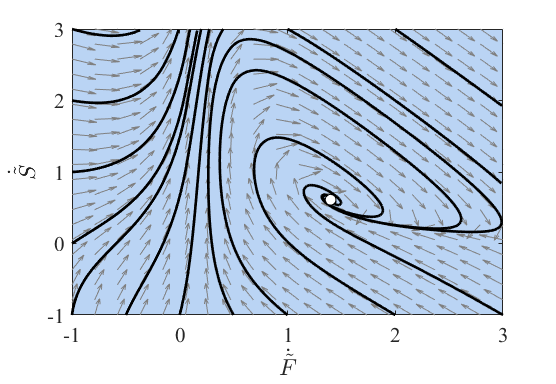
\includegraphics[width = 10cm,trim=5pts 1pts 5pts 17pts, clip]{images/phase_plane.png}
    \caption{Phase plane when $\alpha = 0.2$ and $\beta = 1.2$.}
    \label{fig:phase_plane}
\end{figure}
\vfill
\begin{figure}[H]
    \centering
    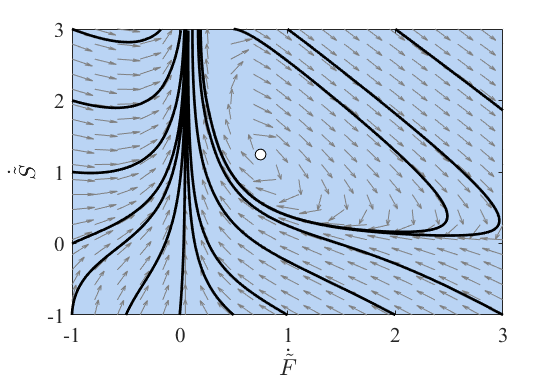
\includegraphics[width = 10cm]{images/phase_plane2.png}
    \caption{Phase plane when $\alpha = 0.05$ and $\beta = 0.7$.}
    \label{fig:phase_plane2}
\end{figure}

\vfill















\section{Turing Instability Regions}\label{turing_regions}
\subsection{Instability with Diffusion}\label{eigenvalue}

The Hopf bifurcation will be used as a threshold for the Turing instability. The system is stable for $\beta-\alpha < (\alpha+\beta)^3$, so it is necessary find the region fitting this constraint where the activator-depletion system {\it with} its diffusion terms is unstable. To examine the system with the diffusion terms, Equation (\ref{eq:W_short}) is revisited. Without diffusion, there was $\dot{W}=\gamma~JW$. With diffusion, there is:

\begin{equation}
\label{eq:W_long}
    \dot{W}=D\Delta_\Gamma W+\gamma~JW ~~~~~~~~\text{with}~~~~ ~~
    D=\left(\begin{matrix} 
    1 & 0 \\ 0 & \delta
    \end{matrix}\right)
\end{equation}
\\
\noindent To turn this into a linear system, we can define the following eigenvalue problems to use as substitutes into Equation (\ref{eq:W_long}):

\begin{equation}
\label{eq:sub}
    \dot{W}=\lambda W ~~~~~\text{and}~~~~~ \Delta_\Gamma W = -k^2W
\end{equation}

\pagebreak

\noindent Here, we need $k\neq0$, for diffusion to affect the model. We are concerned with finding constraints on the eigenvalues in $\lambda$. In Section (\ref{analytic}), we will solve these definitions analytically. For now, it is necessary to examine the linear system:
\begin{equation}
    \lambda W = -Dk^2 W+\gamma JW
\end{equation}
\noindend Once the characteristic equation for $\lambda$ is found, it will provide constraints on the parameters $\alpha, ~\beta, ~\gamma,$ and $\delta$ that will ensure instability, and thus reveal the Turing region. Instability without diffusion required the eigenvalues produced by the Jacobian matrix be negative. With diffusion, the goal is to find at least 1 positive eigenvalue. The characteristic equation is found in the same way as seen in Section (\ref{fixed_points}):
$$    \det(  - Dk^2 + \gamma~J-\lambda I ) = 0 ~~~~~ \longrightarrow ~~~~~  \det(X-\lambda I)=0 ~~~~~ \longrightarrow$$
\begin{equation}
    \label{linear}
    \det\left[\left(\begin{matrix}
        -k^2+\gamma f_F & \gamma f_S \\
        \gamma s_F & -\delta k^2 + \gamma s_S
        \end{matrix}\right)-\lambda I\right]=0
\end{equation}
\\
 \noindent Here, $f_f, ~f_S, ~s_F,$ and $s_S$ are assumed to be evaluated at the fixed point $(F^*,S^*)$. Now we can utilize the equation $\lambda^2-\lambda\text{tr}(X)+\det(X)=0$, yielding:

\begin{equation}
\label{eq:quad}
    \begin{aligned}
        \lambda^2 - \lambda[\gamma~(f_F+s_S)&-k^2(1+\delta)] + \text{det}(X)=0 \\
        \text{Where } ~ \text{det}(X) = \delta k^4-\gamma&(\delta f_F + s_S)k^2 + \gamma^2(f_Fs_s-f_ss_F) \\
    \end{aligned}
\end{equation}
\\
A value satisfying det$(X)<0$ is desired, because it will ensure that the fixed point becomes an unstable saddle node. Alternatively, we could constrain tr($X)>0$ to ensure instability, however we have already established that $f_F+s_S<0$ (\ref{eq:constraints_generic}). Thus tr$(X)<0$, and we must focus on the parameter values that satisfy det$(X)<0$. 

We can examine each term in det$(X)$ to determine the deciding factors for instability. We know that $\delta k^4$ must always be positive, since $\delta>0$. Also, since $\gamma^2(f_Fs_S-f_Ss_F)$ is equal to $\gamma^2$det$(J)$, it must be positive, as this was a constraint established on the system without diffusion. The coefficient of interest is $\gamma(\delta f_F+s_S)k^2$, which must be positive for det$(X)<0$. We already know that $f_F+s_S<0$ (\ref{eq:constraints_generic}) and $s_S<0$ (\ref{eq:J}). Constraining $f_F$ to be positive, we can change the sign of this term. This requires $\alpha<\beta$ and $ \delta(\beta-\alpha) > (\alpha+\beta)^3$, although this will not be sufficient to fulfill all the needed constraints. In addition, we must make this term large enough to shadow its positive neighbors, so we need $\delta>\delta_c$ for some critical value $\delta_c>1$. This critical value is found by solving det$(X)$=0.

We now know that for instability to occur, we need to find the threshold for $\delta$ that makes the $\gamma$ coefficient term in det$(X)$ larger that the other two terms, as well as restrict the parameters $\alpha$ and $\beta$ so that $f_F$ is positive. This constraint is apparent when examining the form of (\ref{eq:lambda}), as a negative value for the determinant ensures one eigenvalue will be positive and one will be negative. The threshold for $\delta_c$ can be found by taking the derivative of det$(X)$ with respect to $k^2$, and examining the region where the minimum is negative.
\begin{equation}
\label{eq:kval}
    2\delta_c k^2-\gamma(\delta_c f_F+s_S) = 0 ~~~~~~~~~~ \longrightarrow ~~~~~~~~~~ k^2 = \gamma\frac{\delta_c f_F+s_S}{2\delta_c}
\end{equation}

\noindent Next, we plug this value into det$(X)$=0 and solve for $\delta_c$:
\\
\begin{equation}
    \label{eq:min}
    \begin{aligned}
     &4\delta_c(f_Fs_S-f_Ss_F)-(\delta_c f_F+s_S)^2 = 0  ~~~~~~ \longrightarrow\\
     %&f_F^2\delta_c^2 -(2f_Fs_S-4f_Ss_F)\delta_c+ s_S^2 =0 ~~~~~~~~ \longrightarrow\\
     %\\
     & \left(\frac{}{}\delta_c(\beta-\alpha)-(\alpha+\beta)^3\right)^2 = 4\delta_c(a+b)^4 \\
    \end{aligned}
\end{equation}
\\
These parameter constraints describe Turing regions in terms of $\alpha$, $\beta$, and $\delta$. They also provide a minimum delta value, specifically:

\begin{equation}
    \label{delta_c}
    \delta_c = \frac{(\alpha+\beta)^2}{\beta-\alpha}\left(\alpha+3\beta-\sqrt{(\alpha+3\beta)^2-4(\beta-\alpha)}\right)
\end{equation}


The wave number $k^2$ is also critical. Variations can effect the instability that depends on det$(X)<0$. The critical values of $k$ are found when det$(X)=0$, as in (\ref{eq:quad}). Since det$(X)$ is degree 2 polynomial with respect to $k^2$, we can apply the quadratic formula to find the critical wave numbers. This yields:
\\
\begin{equation}
    \label{kcrit}
    \begin{aligned}
        k &= \frac{\gamma}{2\delta}\left((\delta f_F+s_S) \pm \sqrt{(\delta f_F+s_S)^2 - 4\delta(f_Fs_S - f_Ss_F)}\right)~~~~~~~~~~~~~~~ \\
    \end{aligned}
\end{equation}
\\
$$ ~~~~~~~=\frac{\gamma}{2\delta}\left(\delta\left(\frac{\beta-\alpha}{\alpha+\beta}\right) -(\alpha+\beta)^2\pm \sqrt{\delta^2\left(\frac{\beta-\alpha}{\alpha+\beta}-(\alpha+\beta)^2\right)^2-4\delta(\alpha+\beta)^2}\right)$$

\noindent We then have $k_{min} < k < k_{max}$. More about the wave number will be discussed in Section \ref{analytic}.

















\subsection{Parameter Values Summary}\label{summary}

There are now multiple constraints on $\alpha$, $\beta$, and $\delta$ that define the Turing instability region. These are summarized in Table (\ref{tab:constraints}) below. We can also visualize these regions for various values of $\delta$, as shown in Figure (\ref{fig:instability_region}). The blue area is a Turing Instability Region. Notice that the region grows for increasing $\delta$, and for $\delta>>1$, the slope at the origin tends toward $\alpha = \beta$.

\vspace{4mm}

\begin{table}[H]
    \centering
    \begin{tabular}{|c | c | c|}
    \hline
        \textbf{Generic Constraint}  & \textbf{Parameter Constraint} \\
        \hline
        $f_F+s_s<0$ & \beta-\alpha < (\alpha+\beta)^3 \\ 
        \hline
        \delta $f_F + s_S >0$ & \alpha < \beta ~~\text{and}~~ \delta(\beta-\alpha) > (\alpha+\beta)^3 \\
        \hline
        4\delta_c(f_Fs_S-f_Ss_F)-(\delta_c f_F+s_S)^2 > 0 & \left(\frac{}{}\delta(\beta-\alpha)-(\alpha+\beta)^3\right)^2 > 4\delta(a+b)^4 \\
        \hline
    \end{tabular}
    \caption{Parameter Constraints for Turing Instability}
    \label{tab:constraints}
\end{table}

\vfill

\begin{figure}[H]
\centering
    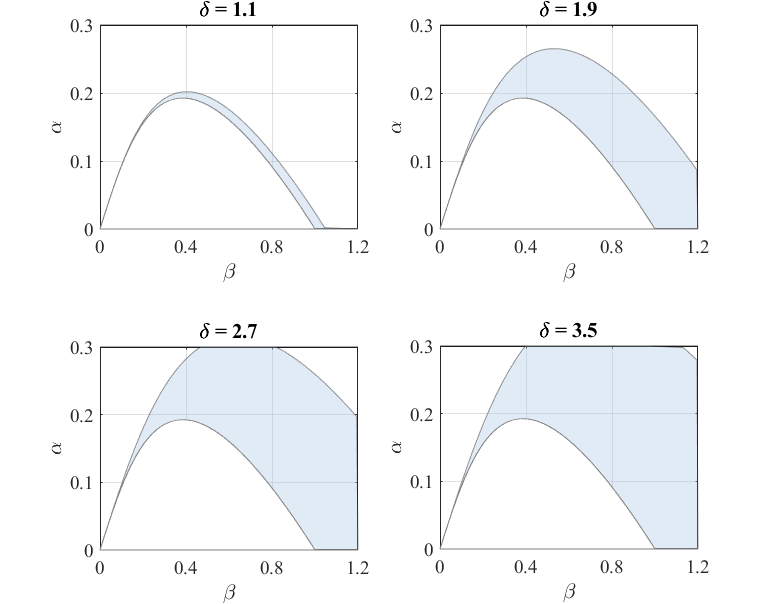
\includegraphics[width = 12cm,trim=35pts 0pts 15pts 0pts, clip]{images/delta_parameters.png}
    \caption{Instability region for varying $\delta$.}
    \label{fig:instability_region}
\end{figure}













\subsection{Analytic Solution}\label{analytic}

Having established several parameter constraints, we can now solve the eigenvalue problems stated in (\ref{eq:sub}). Since the domain is the surface of a sphere, the following boundary conditions and initial conditions are set as:

$$ t>0, ~~~ r=1, ~~~ -\frac{\pi}{2}<\phi<\frac{\pi}{2}, ~~~ -\pi<\theta<\pi, ~~~ \text{and} ~~~ W(\phi,\theta,0) = (F^*,S^*)^T $$

\noindent The following analysis will a few considerations into account, primarily that $W$ is homogeneous and separable, which we know is not always the case. For the analytic solution to this model, we can make these assumptions. 

To solve the eigenvalue problems, we solve their corresponding eigenfunctions. The time dependent eigenvalue problem is already a simple ODE that is readily solved by an exponential function, which has the solution $e^{\lambda t}$. The values for $\lambda$ can be found from using the quadratic equation on (\ref{eq:quad}). Since we set the parameters to produce one positive and one negative real eigenvalue, there is one value of $\lambda$ that produces exponential growth and one that produces exponential decay. The nature of the biological application indicates that the solution must decay, as lung growth naturally slows over time. We can then eliminate the positive eigenvalue from the solution, so $e^{\lambda}$ is defined for negative $\lambda$.

The Laplace-Beltrami eigenvalue problem takes a 3-dimensional argument in spherical coordinates and eliminates the dependence on the radial vector. If we assume that our solution has the form $ W(\phi,\theta,t)=x(\phi)y(\theta)z(t) $, the result is the two Sturm-Liouville equations:

\begin{equation*}
    \frac{d}{d\phi}\left(\sin{\phi}x'(\phi)\right)+\left(k^2\sin{\phi}-\frac{\mu}{\sin{\phi}}\right)x(\phi)=0 
    ~~~~~~ \text{and} ~~~~~~
    y''(\theta) - \mu y(\theta) = 0
\end{equation*}
\\
\noindent We find periodic solution for $y(\theta)$, since $y(\pi)=y(-\pi)$, and likewise for the derivative $y'(\theta)$. This leads to solutions in sine and cosine. The function in $x(\phi)$ is the Legendere equation. We now have the 3 eigenfunctions for $W$ in $t$, $\phi$, and $\theta$:

\begin{equation}
\label{eigenfunctions}
    x_{mn}(\phi)=P_n^m(\cos{\phi})~,~~~~~ y_m(\theta)=e^{im\theta}~,~~~~ \text{and} ~~~~ z_{mn}(t)=e^{\lambda t}
    \end{equation} 
    
\noindent with $m=0,1,2,...$ and $n\geq m$. The eigenvalue $\mu$ is equal to $m^2$. The wave numbers are necessarily $k=\pm \sqrt{n(n+1)}$, which satisfied the the Legendre Polynomial in $\phi$. Together, the eigenfunctions in $x$ $y$ are define as the spherical harmonics $Y_n^m(\phi,\theta) = P_n^m(\cos{\phi})e^{im\theta}$, and have many applications in dynamical systems.\cite{Frye2012} Since we already established an interval for $k$ in which the Turing Region exists, we can define the solution in terms of the maximum and minimum values of $k$. Let $k_1$ designate the smallest integer value in $(k_{min},k_{max})$, and let $k_2$ be the greatest integer value in $(k_{min},k_{max})$. Then the analytical solution can be defined as:

\\
\begin{equation}
\label{asol}
    \begin{aligned}
        W(\phi,\theta,t)=\sum_{m=0}^\infty ~~\sum_{n=k_{1}\geq m}^{k_{2}} e^{\lambda t}Y_n^m(\phi,\theta) \\
        \text{with} ~~~ A_{mn}=\frac{\int_0^\pi\int_{-\pi}^\pi \left(_{S^*}^{F^*}\right)Y_n^m(\phi,\theta)\sin{\phi}d\theta d\phi}{\int_0^\pi\int_{-\pi}^\pi [Y_n^m(\phi,\theta)]^2\sin{\phi}d\theta d\phi}\\
    \end{aligned}
\end{equation}
\\

       

Considering all the parameter constraints, this solution can be quite complex. Even more analysis can be done to specify the wave numbers under values of $\delta$. For $\delta$ close to 1, the wave number interval may not contain an integer. A more detailed investigation into this model in the bulk of a 3D volume under Cartesian coordinates can be found in J.D. Murray's \textit{Mathematical Biology II}.\cite{MurrayII2003}

\section{Discussion of Results}\label{discussion}

If we relate the results of this analysis back to the genetic expression of FGF10 and SHH, there are some interesting conclusions about how these morphogens interact. First, $\alpha<\beta$ indicates that the system must begin with higher amounts of the inhibitor SHH. Logically, this is necessary to insure that lung growth does not occur too quickly. Also, the constraint $\delta>1$ indicates that SHH must diffuse faster than FGF10. We can see that SHH's role as the inhibitor is vital; considering it needs high initial concentrations and high diffusion rates in order to regulate the system.
\pagebreak

Although the analytical solution was found and the constraints are known, no 3D visualization was created. While other researchers have successfully done so both numerically and analytically,\cite{Murray2002}\cite{Varea1999}\cite{murphyL} The lack of context in biological systems makes for weak speculations. Therefore, such images have been omitted. The relationship between FGF10 and SHH may be explained by the mechanisms described in this paper, however this will only be known after solving on a growing domain. Solving on an ellipsoid may be more relevant, but the purpose of this analysis is to gain an understanding about \textit{how} patterns form via chemical reactions, which can be applied to lung development when the domain is a more complex structure. 

This research is only a small stepping stone to an investigation into human lung formation. An analysis of this model on a growing 3D mesh of the human lung is the ultimate goal. However, there is no analytical solution to such complex geometries, so the finite element method will be employed using the C++ library $deal.ii$. There is still much to research to explore in this topic, and this specific application has not yet been done.

\section{Conclusion}\label{conclusion}

Although this line of research is ripe for analysis, the methodologies are not without criticism. Many biologists disapprove of Turing's methods, because they apply to so few biological systems. Lung branching is one such system, however it is still unknown \textit{why} Turing analysis explains this phenomena. The highly complex interaction between many genes during fetal development hides the subtle influences that may contribute to lung branching, and current biological research has not yet been able to observe these interactions \textit{in utero}. 

While Turing's theories on reaction-diffusion systems are likely not the only explanation for pattern formation in this context, they may many applications to offer and perhaps even more not yet explored. Particularly, there may be a possibility for treating Congenital Diaphragmatic Hernias (CDH), which causes hypoplastic lung development in the fetus. Current treatment options have low success rates, but more research will help pediatricians provide better treatment options. With the rapid advances in technology we see every year, perhaps soon we will be able to provide gene therapy to regrow undeveloped lungs, or even make artificial ones. For now, we can take small but important steps towards these goals.


\pagebreak

%\nocite{*}
\bibliographystyle{ieeetr}
\bibliography{Total_04_23.bib}


\end{document}























 